%!TEX root = ../resources/csv/resources/csv/../resources/csv/resources/csv/../resources/csv/resources/csv/tugas-akhir.tex
\section{Evaluasi}
  \subsection{Tujuan Pengujian}
    Pada penelitian ini pengujian dilakukan untuk melakukan evaluasi apakah modifikasi terhadap perangkat OpenSSL merupakan modifikasi yang baik. Pengujian dilakukan terhadap dua bagian dari OpenSSL, yaitu pengujian terhadap fungsionalitas OpenSSL serta pengujian terhadap kinerja OpenSSL.

    Pengujian fungsional dilakukan untuk memastikan bahwa fungsionalitas dari OpenSSL tetap berjalan dengan baik setelah dilakukan modifikasi terhadap \textit{source code}. Pengujian fungsional dilakukan terhadap operasi artimatika big integer yang telah diubah untuk memastikan hasil dari operasi aritmatika tersebut masih merupakan hasil yang benar.

    Pengujian kinerja dilakukan untuk menjawab rumusan masalah poin pertama dan ketiga pada subbab \ref{sec:rumusan_masalah}. Pengujian kinerja akan menjawab apakah kinerja TLS dapat meningkat setelah menggunakan algoritma paralel dalam operasi aritmatika big integer. Selain itu, pengujian kinerja akan menunjukkan apakah algoritma paralel yang digunakan dalam operasi aritmatika merupakan algoritma yang tepat atau tidak.

  \subsection{Pengujian Fungsional} \label{sec:func_testing}

    \subsubsection{Lingkungan Pengujian}
      Lingkungan pengujian yang digunakan dalam pengujian fungsional sama dengan lingkungan implementasi yang telah dijelaskan dalam \ref{sec:impl_env} namun tanpa penggunaan Apache sebagai web server. Pengujian fungsional hanya membutuhkan \textit{source code} OpenSSL serta testcase yang digunakan.

    \subsubsection{Skenario Pengujian}
      % OpenSSL udah punya tc
      OpenSSL telah memiliki kakas yang dapat dilakukan untuk melakukan unit test. Kakas yang digunakan merupakan gabungan dari \textit{perl script} dan kode dalam bahasa C. \textit{Perl script} akan menjalankan kode dalam bahasa C dan memberikan kasus uji yang sesuai untuk pengujian yang dilakukan. Kode dalam bahasa C akan melakukan \textit{parsing} terhadap kasus uji yang ada, menjalakan fungsi tertentu, kemudian mencocokkan hasil dari fungsi tersebut terhadap kasus uji yang diberika.

      % jelasin gimana cara run -> makefile
      Pengujian fungsional dilakukan melalui makefile dengan command |make test|. Pengujian dilakukan setelah build aplikasi selesai dilakukan, namun sebelum dilakukannya instalasi aplikasi pada sistem. Command |make test| melakukan pengujian terhadap seluruh fungsionalitas OpenSSL, mulai dari library big integer, komputasi kriptografi, sistem sertifikat, serta pembuatan koneksi TLS.

      % testcase yang dipilih kayak gimana, kenapa
      Kasus uji untuk setiap operasi aritmatika disimpan pada |openssl/test/recipes/10-test_bn_data|. Kasus uji untuk setiap operasi aritmatika memiliki file terpisah dengan operasi artimatika yang lain. Sebagai contoh, kasus uji untuk operasi perkalian disimpan pada file |bnmul.txt| pada direktori pengujian. Contoh kasus uji yang digunakan untuk pengujian fungsional dapat dilihat pada Lampiran \ref{sec:functional_testcase}.

    \subsubsection{Hasil Pengujian}
      Pengujian fungsionalitas pada OpenSSL berhasil dilakukan. Tidak ada fungsionalitas dari OpenSSL yang rusak setelah dilakukan modifikasi pada \textit{source code} OpenSSL.
      % \textit{Output} dari pengujian fungsional yang dilakukan dapat dilihat pada Lampiran XXX. \todo{tambahin}

  \subsection{Pengujian Kinerja}

    \subsubsection{Lingkungan Pengujian}

      Kakas yang digunakan untuk testing adalah ApacheBench. Sesuai dengan namanya, ApacheBench dapat melakukan benchmarking pada web server. ApacheBench (ab) akan mengirim sejumlah request dan menghasilkan data kinerja web server yang dipilih. Data yang dihasilkan pleh ab diantaranya adalah jumlah byte yang dikirim antar web server dan ab, jumlah request per detik yang dapat ditangani server, waktu rata-rata yang digunakan untuk menangani sebuah request, serta waktu maksimum dan minimum yang digunakan dalam sebuah request.

      Pengujian dilakukan pada \textit{cloud provider} DigitalOcean. Cloud dipilih karena proses pembuatan server on-demand dengan spesifikasi tertentu dapat dilakukan dengan mudah dan dalam waktu yang singkat. Penggunaan server dengan jumlah core yang tinggi yang dibutuhkan dapat dilakukan dengan menggunakan DigitalOcean CPU-Optimized Droplet. Droplet tersebut mendapatkan dedicated CPU sehingga komputasi paralel pada OpenSSL dapat berjalan dengan menggunakan CPU pada kapasitas maksimum. Arsitektur yang digunakan pada pengujian dapat dilihat pada Gambar \ref{fig:testing_arch}.

      \begin{figure}[h]
        \centering
        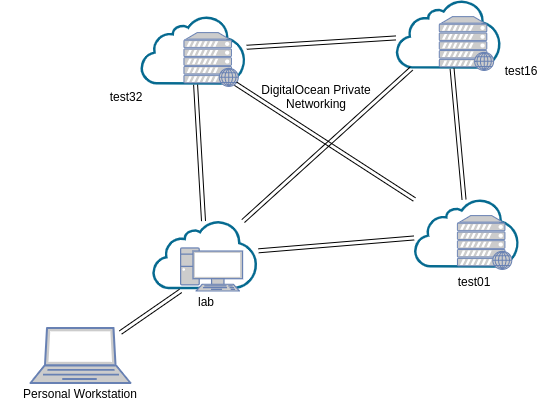
\includegraphics[width=0.8\textwidth]{resources/img/ch-4/testing_arch.png}
        \caption{Arsitektur Lingkungan Pengujian}
        \label{fig:testing_arch}
      \end{figure}

      Pengujian menggunakan empat Droplet, yaitu lab, test01, test16, dan test32. Setiap droplet terhubung melalui DigitalOcean Private Networking, dengan demikian latency antar droplet dapat dikurangi hingga seminimum mungkin. Droplet test01, test16, dan test32 merupakan droplet tempat diinstallnya Apache dan OpenSSL. Arsitektur aplikasi yang terinstall pada test01, test16, dan test32 sama dengan arsitektur implementasi pada Gambar \ref{fig:openssl_arch}. Droplet lab digunakan sebagai tempat melakukan testing dan tempat dijalankannya kakas ApacheBench. Komunikasi antar droplet lab dan personal workstation dilakukan dengan ssh. Tabel \ref{tab:droplet_specs} menjelaskan spesifikasi yang dimiliki setiap droplet.

      \begin{table}[]
        \caption{Spesifikasi Droplet} % title of Table
        \label{tab:droplet_specs}
        \centering % used for centering table
        \begin{tabular}{@{}rcccc@{}}
          \toprule
          \multicolumn{1}{c}{\textbf{Spesifikasi}} & \textbf{lab} & \textbf{test01} & \textbf{test16} & \textbf{test32} \\ \midrule
          \textbf{vCPU}                            & 1            & 1               & 16              & 32              \\
          \textbf{Memori (GB)}                     & 1            & 1               & 32              & 64              \\
          \textbf{SSD Disk (GB)}                   & 25           & 25              & 200             & 400             \\ \bottomrule
        \end{tabular}
      \end{table}

    \subsubsection{Skenario Pengujian}
      Pengujian kinerja dibagi menjadi dua bagian besar. Bagian pertama adalah pengujian kinerja terhadap setiap fungsi yang ada dalam library big integer, sementara bagian kedua adalah pengujian kinerja terhadap penggunaan library dalam website yang menggunakan HTTPS.

      \subparagraph{Pengujian Library}
      Pengujian library dilakukan terhadap beberapa fungsi dalam libcrypto, yaitu beberapa fungsi dalam modul |bn| serta modul |rsa| dan |dh| yang menggunakan operasi aritmatika big integer dalam modul crypto. Setiap pengujian dilakukan terhadap satu variabel yang berbeda, variabel tersebut dapat dilihat pada grafik yang ada.

      \subparagraph{Pengujian HTTPS}
      Pengujian HTTPS dilakukan dengan menjalankan ApacheBench pada node lab dengan tujuan web yang dicek test01, test16, dan test32. ApacheBench menghasilkan beberapa data, namun kita hanya peduli pada data berikut.
      % \todo{cite website apachebench}
      \begin{enumerate}[label=\roman*.]
        \item \textit{Time taken for tests}, yaitu waktu dari koneksi pertama dibuat sampai response terakhir diterima.
        \item \textit{Requests per second}, yaitu jumlah request yang ditangani dalam satu detik
        \item \textit{Time per request}, yaitu waktu rata-rata untuk sebuah request.
        \item \textit{Min \& max connection times}, yaitu waktu maksimum dan minimum yang digunakan oleh sebuah request.
      \end{enumerate}

      Pengujian dengan ApacheBench dilakukan terhadap beberapa versi perangkat OpenSSL. Versi pertama adalah OpenSSL vanilla yang belum dimodifikasi, versi kedua adalah OpenSSL dengan paralelisasi modul penjumlahan dan pengurangan, versi ketiga adalah OpenSSL dengan paralelisasi modul perkalian, versi keempat adalah OpenSSL dengan paralelisasi modul pembagian, dan versi kelima adalah OpenSSL dengan semua paralelisasi semua modul operasi aritmatika.

    \subsubsection{Hasil dan Analisis Pengujian}


    \subparagraph{Operasi Penjumlahan}
    \begin{figure}[h]
      \centering
      \begin{tikzpicture}
        \begin{axis}[
            x unit=Kbyte,
            y SI prefix=milli,y unit=s,
            xlabel={Panjang Data},
            ylabel={Waktu}
          ]
          \addplot[color=orange,] table [x expr=\thisrow{tc_num}/(8*1024), y expr=\thisrow{time_avg}/(10^3), col sep=comma] {./resources/csv/bn1_add.csv};
          \addlegendentry{local-1cpu}
          \addplot[color=blue,] table [x expr=\thisrow{tc_num}/(8*1024), y expr=\thisrow{time_avg}/(10^3), col sep=comma] {./resources/csv/bn2_add.csv};
          \addlegendentry{local-2cpu}
          % \addplot[color=red,] table [x expr=\thisrow{tc_num}/(8*1024), y expr=\thisrow{time_avg}/(10^3), col sep=comma] {./resources/csv/do/bn1b_add.csv};
          % \addlegendentry{do-1cpu}
          % \addplot[color=green,] table [x expr=\thisrow{tc_num}/(8*1024), y expr=\thisrow{time_avg}/(10^3), col sep=comma] {./resources/csv/do/bn2b_add.csv};
          % \addlegendentry{do-4cpu}
        \end{axis}
      \end{tikzpicture}
      \caption{Data Penjumlahan}
      \label{fig:data_add}
    \end{figure}

    Grafik \ref{fig:data_add} menggambarkan hasil pengujian untuk operasi penjumlahan. Tidak dilakukan pengujian untuk operasi pengurangan karena grafik yang dihasilkan akan sama dengan operasi penjumlahan. Pada pengujian ini dilakukan  seratus penjumlahan BIGNUM $a + b$ dengan panjang yang diubah dari 2KByte hingga 20KByte dengan jarak antar data 2KByte.

    Grafik yang dihasilkan menunjukkan waktu yang diperlukan merupakan fungsi linear dari panjang data. Hal ini sesuai dengan fungsi penjumlahan yang memiliki kompleksitas $O(n)$. Hasil paralelisasi yang didapat tidak bagus. Overhead yang didapat dari pembuatan thread masih lebih besar dibandingkan dengan percepatan yang didapat, bahkan pada panjang data 20KByte. Hal ini terjadi karena operasi yang terdapat pada operasi ini hanyalah operasi penjumlahan saja.

    \subparagraph{Operasi Perkalian}
    \begin{figure}[h]
      \centering
      \begin{tikzpicture}
          \begin{axis}[
              x unit=Kbyte,
              y SI prefix=milli,y unit=s,
              xlabel={Panjang Data},
              ylabel={Waktu}
            ]
          \addplot[color=orange,] table [x expr=\thisrow{tc_num}/(8*1024), y expr=\thisrow{time_avg}/(10^3), col sep=comma] {./resources/csv/bn1b_mul.csv};
          \addlegendentry{local-1cpu}
          \addplot[color=blue,] table [x expr=\thisrow{tc_num}/(8*1024), y expr=\thisrow{time_avg}/(10^3), col sep=comma] {./resources/csv/bn2b_mul.csv};
          \addlegendentry{local-2cpu}
          % \addplot[color=red,] table [x expr=\thisrow{tc_num}/(8*1024), y expr=\thisrow{time_avg}/(10^3), col sep=comma] {./resources/csv/bn1b_sqr.csv};
          % \addlegendentry{do-2cpu}
          % \addplot[color=green,] table [x expr=\thisrow{tc_num}/(8*1024), y expr=\thisrow{time_avg}/(10^3), col sep=comma] {./resources/csv/do/bn2b_mul.csv};
          % \addlegendentry{do-4cpu}
        \end{axis}
      \end{tikzpicture}
      \caption{Data Perkalian Panjang}
      \label{fig:data_mul}
    \end{figure}

    Grafik \ref{fig:data_mul} menggambarkan hasil pengujian untuk operasi perkalian dengan algoritma perkalian panjang. Pada pengujian ini dilakukan seratus perkalian BIGNUM $a * b$ dengan panjang yang diubah dari 64Byte hingga 6,4KByte dengan jarak antar data 64Byte.

    Operasi perkalian panjang memiliki kompleksitas $O(n^2)$, hal ini terlihat dari grafik bahwa fungsi waktu merupakan fungsi kuadratik terhadap panjang data. Terlihat pada grafik bahwa fungsi dengan paralelisasi awalnya memiliki waktu yang lebih lambat dibandingkan fungsi awal. Pada panjang data 1KByte, fungsi paralel sudah mulai memberikan hasil yang lebih cepat dibandingkan dengan data awal. Waktu yang dihasilkan oleh fungsi paralel lebih tidak stabil dibandingkan dengan fungsi non paralel, hal ini terjadi karena perlunya dilakukan alokasi memori tambahan untuk setiap thread yang dibuat, sementara itu alokasi memori tidak memiliki waktu eksekusi yang konsisten.

    \begin{figure}[h]
      \centering
      \begin{tikzpicture}
          \begin{axis}[
              x unit=Kbyte,
              y SI prefix=milli,y unit=s,
              xlabel={Panjang Data},
              ylabel={Waktu}
            ]
          \addplot[color=orange,] table [x expr=\thisrow{tc_num}/(8*1024), y expr=\thisrow{time_avg}/(10^3), col sep=comma] {./resources/csv/bn1b_mul_recursive.csv};
          \addlegendentry{local-1cpu}
          \addplot[color=blue,] table [x expr=\thisrow{tc_num}/(8*1024), y expr=\thisrow{time_avg}/(10^3), col sep=comma] {./resources/csv/bn2b_mul_recursive.csv};
          \addlegendentry{local-2cpu}
          % \addplot[color=red,] table [x expr=\thisrow{tc_num}/(8*1024), y expr=\thisrow{time_avg}/(10^3), col sep=comma] {./resources/csv/do/bn1b_mul_recursive.csv};
          % \addlegendentry{do-1cpu}
          % \addplot[color=green,] table [x expr=\thisrow{tc_num}/(8*1024), y expr=\thisrow{time_avg}/(10^3), col sep=comma] {./resources/csv/do/bn2b_mul_recursive.csv};
          % \addlegendentry{do-4cpu}
        \end{axis}
      \end{tikzpicture}
      \caption{Data Perkalian Karatsuba}
      \label{fig:data_mul_recursive}
    \end{figure}

    Grafik \ref{fig:data_mul_recursive} menggambarkan hasil pengujian untuk operasi perkalian dengan algoritma perkalian panjang. Pada pengujian ini dilakukan seratus perkalian BIGNUM $a * b$ dengan panjang yang diubah dari 64Byte hingga 6,4KByte dengan jarak antar data 64Byte.

    Seperti data perkalian panjang, data fungsi paralel tidak stabil karena dilakukan alokasi memori untuk setiap kali pemanggilan thread. Fungsi perkalian karatsuba paralel mulai lebih cepat dibandingkan dengan fungsi non-paralel mulai dari panjang data 2KB. Hal ini terjadi karena overhead pemanggilan thread secara rekursif lebih tinggi dibandingkan dengan pemanggilan thread biasa.

    \subparagraph{Operasi Perpangkatan Dua}


    \begin{figure}[h]
      \centering
      \begin{tikzpicture}
          \begin{axis}[
              x unit=Kbyte,
              y SI prefix=milli,y unit=s,
              xlabel={Panjang Data},
              ylabel={Waktu}
            ]
          \addplot[color=orange, ] table [x expr=\thisrow{tc_num}/(8*1024), y expr=\thisrow{time_avg}/(10^3), col sep=comma] {./resources/csv/bn1b_sqr.csv};
          \addlegendentry{local-1cpu}
          \addplot[color=blue,] table [x expr=\thisrow{tc_num}/(8*1024), y expr=\thisrow{time_avg}/(10^3), col sep=comma] {./resources/csv/bn2b_sqr.csv};
          \addlegendentry{local-2cpu}
          % \addplot[color=red,] table [x expr=\thisrow{tc_num}/(8*1024), y expr=\thisrow{time_avg}/(10^3), col sep=comma] {./resources/csv/do/bn1b_sqr.csv};
          % \addlegendentry{do-1cpu}
          % \addplot[color=green,] table [x expr=\thisrow{tc_num}/(8*1024), y expr=\thisrow{time_avg}/(10^3), col sep=comma] {./resources/csv/do/bn2b_sqr.csv};
          % \addlegendentry{do-4cpu}
        \end{axis}
      \end{tikzpicture}
      \caption{Data Perpangkatan Dua}
      \label{fig:data_sqr}
    \end{figure}

    Grafik \ref{fig:data_sqr} menggambarkan hasil pengujian untuk operasi perkalian dengan algoritma perkalian panjang. Pada pengujian ini dilakukan seratus perpangkatan dua BIGNUM $a^2$ dengan panjang yang diubah dari 64Byte hingga 6,4KByte dengan jarak antar data 64Byte.

    Tidak dilakukan paralelisasi khusus untuk operasi ini, namun penulis menemukan bug pada fungsi perpangkatan dua di OpenSSL. Pada fungsi awalnya, hanya dilakukan perkalian karatsuba hanya pada bilangan yang memiliki panjang bilangan pangkat dua. Selain itu akan dilakukan perkalian panjang yang dimodifikasi untuk perpangkatan dua. Karena perkalian karatsuba lebih efektif, maka penulis mengubah fungsi perpangkatan dua untuk memanggil fungsi perkalian karatsuba |bn1_mul_recursive()|. Karena itulah grafik yang didapat mirip dengan hasil perkalian karatsuba pada grafik \ref{fig:data_mul_recursive}.

    \subparagraph{Operasi Perkalian Modular}
    \begin{figure}[h]
      \centering
      \begin{tikzpicture}
          \begin{axis}[
              x unit=Kbyte,
              y SI prefix=milli,y unit=s,
              xlabel={Panjang Data},
              ylabel={Waktu}
            ]
          \addplot[color=orange,] table [x expr=\thisrow{tc_num}/(8*1024), y expr=\thisrow{time_avg}/(10^3), col sep=comma] {./resources/csv/bn1b_modmul.csv};
          \addlegendentry{local-1cpu}
          \addplot[color=blue,] table [x expr=\thisrow{tc_num}/(8*1024), y expr=\thisrow{time_avg}/(10^3), col sep=comma] {./resources/csv/bn2b_modmul.csv};
          \addlegendentry{local-2cpu}
          % \addplot[color=red,] table [x expr=\thisrow{tc_num}/(8*1024), y expr=\thisrow{time_avg}/(10^3), col sep=comma] {./resources/csv/do/bn1b_modmul.csv};
          % \addlegendentry{do-1cpu}
          % \addplot[color=green,] table [x expr=\thisrow{tc_num}/(8*1024), y expr=\thisrow{time_avg}/(10^3), col sep=comma] {./resources/csv/do/bn2b_modmul.csv};
          % \addlegendentry{do-4cpu}
        \end{axis}
      \end{tikzpicture}
      \caption{Data Perkalian Modular}
      \label{fig:data_modmul}
    \end{figure}

    Grafik \ref{fig:data_modmul} menggambarkan hasil pengujian untuk operasi perkalian dengan algoritma perkalian panjang. Pada pengujian ini dilakukan seratus perkalian modular BIGNUM $a*b \mod m$ dengan panjang $a$ dan $b$ yang diubah dari 64Byte hingga 6,4KByte dengan jarak antar data 64Byte.

    Perkalian modular $a*b \mod m$ dilakukan dengan melakukan perkalian karatsuba terhadap $a$ dan $b$, kemudian melakukan pembagian hasil perkalian tersebut pada $m$ dan mengambil sisanya. Karena itulah grafik yang didapat mirip dengan grafik perkalian karatsuba. Mirip dengan pengujian sebelumnya, fungsi paralel mulai lebih cepat pada panjang data 2KByte.


    \subparagraph{Operasi Perpangkatan Modular}
    \begin{figure}[h]
      \centering
      \begin{tikzpicture}
          \begin{axis}[
              x unit=Kbyte,
              y unit=s,
              xlabel={Panjang Data},
              ylabel={Waktu}
            ]
          \addplot[color=orange,] table [x expr=\thisrow{tc_num}/(8*1024), y expr=\thisrow{time_avg}/(10^6), col sep=comma] {./resources/csv/bn1b_modexp.csv};
          \addlegendentry{local-1cpu}
          \addplot[color=blue,] table [x expr=\thisrow{tc_num}/(8*1024), y expr=\thisrow{time_avg}/(10^6), col sep=comma] {./resources/csv/bn2b_modexp.csv};
          \addlegendentry{local-2cpu}
          % \addplot[color=red,] table [x expr=\thisrow{tc_num}/(8*1024), y expr=\thisrow{time_avg}/(10^3), col sep=comma] {./resources/csv/do/bn1b_modexp.csv};
          % \addlegendentry{do-1cpu}
          % \addplot[color=green,] table [x expr=\thisrow{tc_num}/(8*1024), y expr=\thisrow{time_avg}/(10^3), col sep=comma] {./resources/csv/do/bn2b_modexp.csv};
          % \addlegendentry{do-4cpu}
        \end{axis}
      \end{tikzpicture}
      \caption{Data Perpangkatan Modular}
      \label{fig:data_modexp}
    \end{figure}

    Grafik \ref{fig:data_modmul} menggambarkan hasil pengujian untuk operasi perkalian dengan algoritma perkalian panjang. Pada pengujian ini dilakukan seratus perpangkatan modular BIGNUM $a^p \mod m$ dengan panjang yang diubah dari 400Byte hingga 6,4KByte dengan jarak antar data 16Byte.

    Fungsi paralel mulai lebih cepat daripada fungsi perpangkatan modular secara eksponensial pada panjang data sekitar 1KB. Variabel yang paling berpengaruh pada perpangkatan modular adalah panjang data modulus. Hal ini terjadi karena proses perkalian dan perpangkatan hanya dilakukan pada range modulus tersebut saja.

      \subparagraph{Proses Pertukaran Kunci Diffie Hellman}
      \begin{figure}[h]
        \centering
        \begin{tikzpicture}
            \begin{axis}[
                x unit=bit,
                y SI prefix=micro,y unit=s,
                xlabel={Panjang Kunci},
                ylabel={Waktu}
              ]
            \addplot [color=blue] table [x=key_size, y=time_avg, col sep=comma] {resources/csv/dh.csv};
            \addlegendentry{test01}
          \end{axis}
        \end{tikzpicture}
        \caption{Data Pertukaran Kunci Diffie Hellman}
        \label{fig:data_dh}
      \end{figure}

      \subparagraph{Proses Enkripsi dan Dekripsi RSA}

        \begin{figure}[h]
          \centering
          \begin{tikzpicture}
              \begin{axis}[
                  x unit=Kbyte,
                  y unit=s,
                  xlabel={Panjang Data},
                  ylabel={Waktu}
                ]
              \addplot[color=orange, mark=x] table [x expr=\thisrow{key_size}/(8*1024), y expr=\thisrow{time_avg}/(10^6), col sep=comma] {./resources/csv/rsa_enc1b.csv};
              \addlegendentry{local-1cpu}
              \addplot[color=blue,mark=o] table [x expr=\thisrow{key_size}/(8*1024), y expr=\thisrow{time_avg}/(10^6), col sep=comma] {./resources/csv/rsa_enc2b.csv};
              \addlegendentry{local-2cpu}
              % \addplot[color=red,] table [x expr=\thisrow{tc_num}/(8*1024), y expr=\thisrow{time_avg}/(10^6), col sep=comma] {./bn9num_modexp.csv};
              % \addlegendentry{num}
              % \addplot[color=green,] table [x expr=\thisrow{tc_num}/(8*1024), y expr=\thisrow{time_avg}/(10^6), col sep=comma] {./bn9numexp_modexp.csv};
              % \addlegendentry{numexp}
            \end{axis}
          \end{tikzpicture}
          \caption{Data RSA encrypt}
          \label{fig:data_rsa_enc}
        \end{figure}

        Seperti data perpangkatan modular, proses enkripsi dan dekripsi RSA paralel mulai lebih cepat pada panjang kunci ~1KB (8096 byte). Hal ini terjadi karena fungsi enkripsi RSA pada dasarnya merupakan operasi perpangkatan modular terhadap plaintext dengan menggunakan private key sebagai eksponen.
